\begin{center} \resizebox{0.95\textwidth}{!}{ 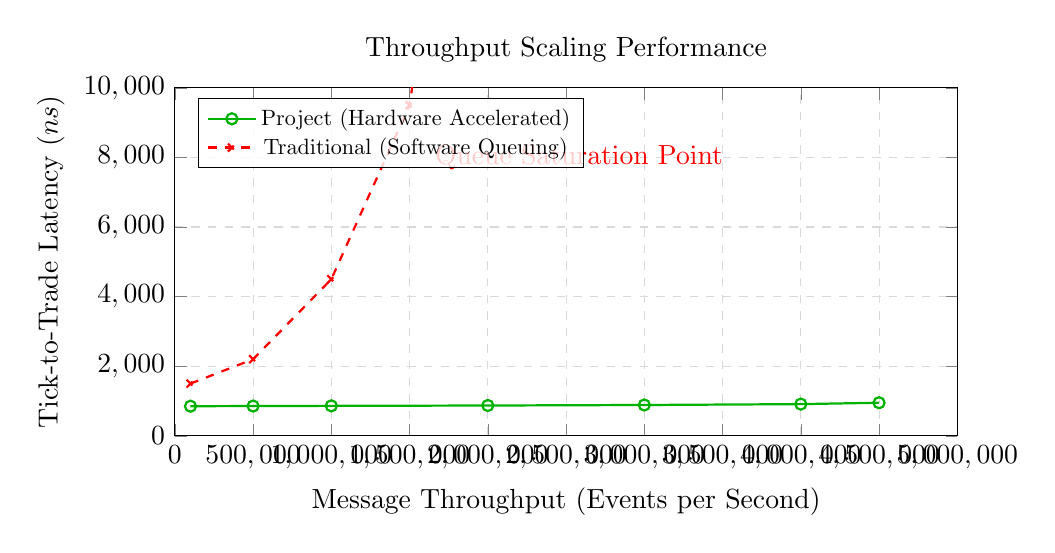
\begin{tikzpicture} \begin{axis}[ width=0.95\columnwidth, height=6cm, xlabel={Message Throughput (Events per Second)}, ylabel={Tick-to-Trade Latency ($ns$)}, xmin=0, xmax=5000000, ymin=0, ymax=10000, grid=major, grid style={dashed, gray!30}, title={Throughput Scaling Performance}, legend pos=north west, legend style={nodes={scale=0.8, transform shape}, fill=white, fill opacity=0.8, draw opacity=1, text opacity=1}, x tick label style={/pgf/number format/fixed, /pgf/number format/1000 sep={,}}, scaled x ticks=false, y tick label style={/pgf/number format/fixed, /pgf/number format/1000 sep={,}}, scaled y ticks=false ] \addplot[color=green!70!black, thick, mark=o] coordinates  { (100000, 850) (500000, 855) (1000000, 860) (2000000, 870) (3000000, 885) (4000000, 910) (4500000, 950) }; \addlegendentry{Project (Hardware Accelerated)} \addplot[color=red, thick, dashed, mark=x] coordinates  { (100000, 1500) (500000, 2200) (1000000, 4500) (1500000, 9500) (2000000, 25000) }; \addlegendentry{Traditional (Software Queuing)} \node[anchor=west, text=red] at (axis cs: 1600000, 8000) {Queue Saturation Point}; \end{axis} \end{tikzpicture} } \end{center}